\begin{BlueBox}
    \vskip-1cm
    \begin{block}{\BHead{Background}}
        \begin{itemize}
            \item Surface temperatures predicted to increase due to climate change.
            \item What are the effects of increased temperatures on air quality?
                \begin{itemize}
                    \item Increased emissions from vegetation (BVOCs).
                    \item Increased reaction rates atmospheric chemistry.
                    \item \ldots
                \end{itemize}
            \vspace{8mm}
            \item Ozone is produced from the photochemistry of emitted \ce{NO_x} and VOC, with VOC being the ``fuel'' and \ce{NO_x} the ``catalyst'' for ozone production.
            \item Due to the photochemical nature of ozone production, meteorological factors such as temperature are drivers for ozone production.
            \item What are the effects of increased temperatures on tropospheric ozone concentrations?
                \begin{itemize}
                    \item Increased VOC emissions, especially BVOCs such as isoprene, are well-known to produce large amounts of ozone per molecule of VOC emitted.
                    \item Increased temperatures means that the PAN sink for peroxy radicals and \ce{NO2} is much less-effective at transporting RO2 and \ce{NO2} away from emission sources due to increased thermal decomposition rates.  
                \end{itemize}
            $\Rightarrow$ Future increases in ozone levels.
        \end{itemize}
        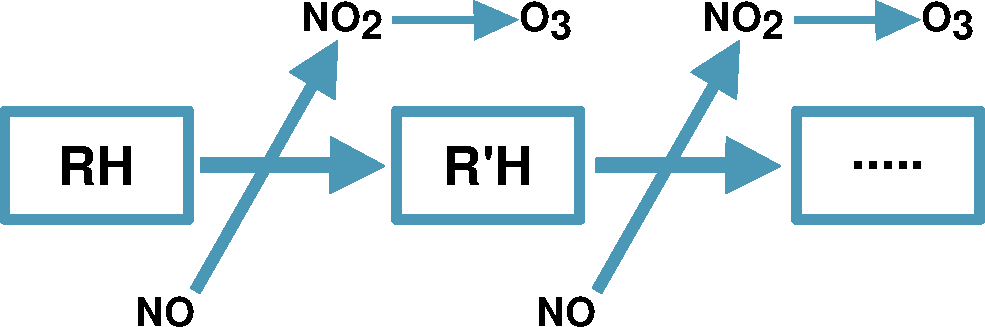
\includegraphics[width=\textwidth]{VOC_Oxidation}
    \end{block}
\end{BlueBox}
